%# -*- coding: utf-8-unix -*-

\chapter{对比实验和结果分析}

\section{实验数据集的选择}

上一章的最后一节已经介绍了KDD Cup 99数据集,并且说明了对数据的预处理步骤,在最后介绍了本文将使用KDD Cup 99数据集中的“KDD 10\%”和“corrected”这两个数据集作为训练和测试数据集。这一节将详细说明一下这两个数据集在实验中各自的用途。

首先,我选择了完整训练数据集的10\%的数据集作为我的训练数据集,考虑了如下两个原因:一是将完整的训练数据集用于训练使得我的训练时间延长了10倍以上(鉴于使用的个人电脑计算能力有限),二是在基于深度学习的网络流量异常检测算法的实现过程中,我在其他参数相同的情况下对比了使用完整训练数据集以及使用完整训练数据集的10\%作为训练数据集的情况下,模型的准确率相当,经完整训练数据集训练后的模型仅仅比使用10\%数据进行训练后的模型的准确率提高了0.001\%,而训练时间却增加了10倍不止。所以,我选择了数据量较为小的数据集作为训练数据集。

关于测试集的选择,阅读了一些文献发现,有一些文献中的测试集选择的同样是训练数据集,只是将训练数据集分割了,其中70\%-75\%的数据用于训练,25\%-30\%的数据用于测试。这种选择虽然在一些其它数据集上很常见,因为其它数据集只有唯一一个训练数据集,但是对于KDD Cup 99数据集来说,我认为应该将corrected数据集作为测试数据集。首先,corrected数据集本身就是设计者专门收集用于测试的,其次,使用包含未知攻击类型的数据集进行测试可以更好的测试我们所构建的模型的泛化能力。从已知攻击类型学习到检测未知攻击类型的异常流量这一能力正是网络流量异常检测算法研究所迫切需要的。当然,也不能否认训练、测试都在训练数据集中的这种方法所体现的机器学习的强大抽象、学习、分类能力。

因此,在实验中我选择使用KDD 10\%的数据对模型进行训练,corrected测试数据集对模型进行测试。同时,在最后的一组实验中,我也给出了使用从训练数据集分割出来部分数据进行测试的准确率。

\section{实验平台}

本章实验是在macOS High Sierra 10.13.4操作系统上进行的,开发语言使用了Python3,Python版本号是3.6.4。硬件平台CPU型号是Intel Core i5-5257U,双核心四线程,CPU主频是2.7GHz,最大可以睿频到3.1GHz,内存为8GB的DDR3内存,内存频率为1867MHz。

\section{实验过程和结果分析}

在对训练数据集和测试数据集预处理后,得到了$494021 \times 122$和$311029 \times 122$维的输入数据。这两组数据将用于对模型的训练和测试。在训练数据中,将随机抽取其中的25\%出来作为验证集。验证集在训练中不会被训练到,仅仅用于调超参数。

本实验进行了多组控制变量的对比实验,在前一个实验当中表现最好的结构将用于下一组实验中,最终通过多组的对比试验构建出表现较为优秀的模型用于网络异常流量检测。

\subsection{模型深度与节点数目的选择}

在本节实验中,本文进行了多次实验,每次实验构建的深度学习网络结构的层数或节点数都是不相同的,通过多次实验的比对,得到了不同层数对应的准确率汇。除了网络参数不同外,其他参数相同,其他参数分别为:
\begin{itemize}
    \item batchsize: 512
    \item dropout: 0(即不使用dropout)
    \item 激活函数: relu
    \item 优化算法: nadam
    \item 损失函数: categorical\_crossentropy
\end{itemize}

测试结果汇总如下:
% Table generated by Excel2LaTeX from sheet 'Sheet2'
\begin{table}[htbp]
	\centering
	\caption{不同网络参数的实验结果}
	\begin{tabular}{c|c|c|c|c}
		\toprule
		模型序号 & 网络参数             & 准确率  & params  & time      \\
		\midrule
		model1-1   & 24-256-512-256-5     & 92.44\% & 273549  & 22s/epoch \\
		\midrule
		model1-2   & 12-128-256-128-5     & 92.10\% & 69705   & 10s/epoch \\
		\midrule
		model1-3   & 48-512-1024-512-5    & 73.90\% & 1083669 & 72s/epoch \\
		\midrule
		model1-4   & 12-24-48-24-5        & 91.99\% & 4289    & 6s/epoch  \\
		\midrule
		model1-5   & 6-12-24-12-5         & 91.44\% & 1499    & 5s/epoch  \\
		\midrule
		model1-6   & 3-6-12-6-5           & 90.86\% & 590     & 5s/epoch  \\
		\midrule
		model1-7   & 24-512-256-5         & 92.32\% & 148365  & 15s/epoch \\
		\midrule
		model1-8   & 24-256-512-256-128-5 & 92.07\% & 305805  & 24s/epoch \\
		\midrule
		model1-9   & 10-50-10-5           & 91.96\% & 2345    & 5s/epoch  \\
		\bottomrule
	\end{tabular}%
	\label{tab:exp1-1}%
\end{table}%

\begin{figure}[H]
    \centering
    \includegraphics[width=0.99\textwidth]{exp1.pdf}
    \caption{网络参数-准确率结果}
    \label{fig:exp1-2}
\end{figure}

\subsection{batchsize大小的选择}

在上一节的实验中,可以发现,模型model1-1的网络参数取得了最好的测试成绩,同时它的训练时间也比较短,故本节实验在model1-1的网络参数的基础上,测试batchsize大小的选择对模型表现的影响。下面的图表是模型的网络参数为“24-256-512-256-5”的基础上不同batchsize的实验结果:
% Table generated by Excel2LaTeX from sheet 'Sheet2'
\begin{table}[htbp]
	\centering
	\caption{不同batchsize的实验结果}
	\begin{tabular}{c|c|c|c}
		\toprule
		模型序号 & batchsize & 准确率  & time       \\
		\midrule
		model2-1 & 512       & 92.12\% & 23s/epoch  \\
		\midrule
		model2-2 & 256       & 92.16\% & 27s/epoch  \\
		\midrule
		model2-3 & 128       & 92.44\% & 37s/epoch  \\
		\midrule
		model2-4 & 64        & 92.24\% & 57s/epoch  \\
		\midrule
		model2-5 & 32        & 92.51\% & 98s/epoch  \\
		\midrule
		model2-6 & 16        & 92.26\% & 185s/epoch \\
		\midrule
		model2-7 & 8         & 92.43\% & 360s/epoch \\
		\midrule
		model2-8 & 1024      & 92.39\% & 20s/epoch  \\
		\midrule
		model2-9 & 2048      & 92.67\% & 19s/epoch  \\
		\bottomrule
	\end{tabular}%
	\label{tab:exp2-1}%
\end{table}%

\begin{figure}[H]
    \centering
    \includegraphics[width=0.99\textwidth]{exp2.pdf}
    \caption{batchsize-准确率结果}
    \label{fig:exp2-2}
\end{figure}

\subsection{优化算法的选择}

在上一节的实验中,可以发现,模型model2-9的batchsize取得了最好的测试成绩,故本节实验在model2-9的batchsize大小以及model1-1的网络参数的基础上,测试不同的优化算法的选择对模型表现的影响。下面的图表给出了不同优化算法对模型表现的影响:
% Table generated by Excel2LaTeX from sheet 'Sheet2'
\begin{table}[htbp]
	\centering
	\caption{不同优化算法的实验结果}
	\begin{tabular}{c|c|c|c}
		\toprule
		模型序号 & 优化算法 & 准确率  & time      \\
		\midrule
		model3-1 & Nadam    & 92.67\% & 19s/epoch \\
		\midrule
		model3-2 & SGD      & 90.67\% & 18s/epoch \\
		\midrule
		model3-3 & RMSprop  & 92.39\% & 19s/epoch \\
		\midrule
		model3-4 & Adagrad  & 91.91\% & 18s/epoch \\
		\midrule
		model3-5 & Adadelta & 91.71\% & 19s/epoch \\
		\midrule
		model3-6 & Adam     & 92.16\% & 19s/epoch \\
		\midrule
		model3-7 & Adamax   & 91.83\% & 19s/epoch \\
		\bottomrule
	\end{tabular}%
	\label{tab:exp3-1}%
\end{table}%

\begin{figure}[H]
    \centering
    \includegraphics[width=0.99\textwidth]{exp3.pdf}
    \caption{优化算法-准确率结果}
    \label{fig:exp3-2}
\end{figure}


\subsection{不同分类精度下模型的表现}

从第三章对KDD Cup 99数据集的介绍中得知,每一条数据都被标记为正常(Normal)或者异常(Attack),异常类型的数据被细分为4大类共39种攻击类型,其中22种攻击类型出现在了训练数据集中,其它的17种未知攻击类型被收纳在测试数据集中。由于有17种类型的攻击数据只在测试集中出现,而在整个模型的实现以及测试过程中,需要对标记数据提前进行编码,所以即使将39种攻击类型都提前编码,在测试时模型也无法输出超出其本身23种(1种正常标记和22种攻击类型标记)编码范围的结果。所以,本实验将数据的标记进行了整理,分为了两种类型:
\begin{enumerate}
    \item 五分类:NORMAL,PROBE,DOS,U2R,R2L这五类标记代表了所有的39种攻击以及正常流量。模型将对输入的数据给出五种之中的一种。
    \item 二分类:Normal,Attack分别用0,1表示。模型只在(0,1)这两个数字中给出结果。也是网络流量异常检测最基本的功能,即区分正常流量和异常流量。
\end{enumerate}

那么,对于五分类以及二分类这两种不同的分类情况,模型的准确率会有很大的差别吗?下面的实验结果给出了答案。在实验中,按原有的网络结构对二分类进行训练得到了准确率仅为80.52\%的结果。在实验中本文尝试了使用不同的模型参数都无法将准确率提升到前几个实验的90\%以上的准确率级别。从第三章我们了解到使用Dropout技术可以克服深度神经网络的训练困难,因此,这里将Dropout技术应用到了模型中,具体的做法是在除输出层外的每一层之后添加Dropout层,Dropout的值设置为了0.5。使用了Dropout技术后继续进行实验,二分类的准确率达到了五分类的同一水准。具体实验数据请看下面的图表:
% Table generated by Excel2LaTeX from sheet 'Sheet2'
\begin{table}[htbp]
	\centering
	\caption{二分类与五分类的实验结果}
	\begin{tabular}{c|c|c|c}
		\toprule
		分类情况 & 准确率  & dropout & 网络参数         \\
		\midrule
		二分类1  & 80.52\% & 0       & 24-256-512-256-1 \\
		\midrule
		二分类2  & 92.04\% & 0.5     & 24-256-512-256-1 \\
		\midrule
		五分类1  & 92.67\% & 0       & 24-256-512-256-5 \\
		\midrule
		五分类2  & 91.66\% & 0.5     & 24-256-512-256-5 \\
		\bottomrule
	\end{tabular}%
	\label{tab:exp4-1}%
\end{table}%

\begin{figure}[H]
    \centering
    \includegraphics[width=0.99\textwidth]{exp4.pdf}
    \caption{不同分类级别-准确率结果}
    \label{fig:exp4-2}
\end{figure}

\subsection{训练与测试同在KDD 10\%数据集的情况}

当使用KDD 10\%数据集的75\%的数据用于训练本文的深度学习模型,使用KDD 10\%数据集的剩余25\%的数据用于测试时,本文的深度学习取得了相当高的准确率,准确率达到了惊人的99.92\%。下面两图为过程中的具体情况:
\begin{figure}[H]
	\centering
	\begin{subfigure}{.45\textwidth}
		\centering
		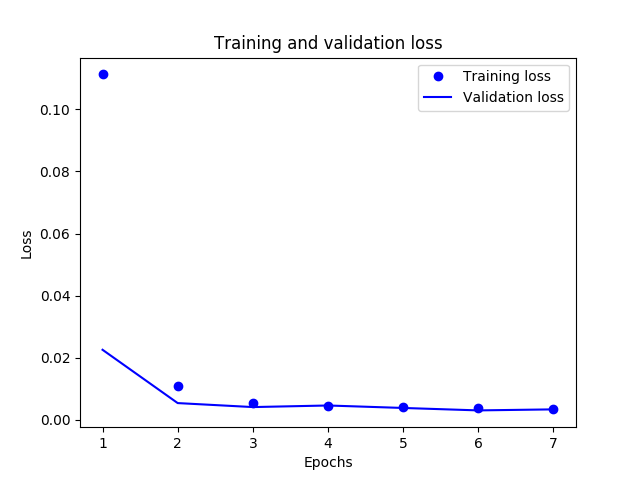
\includegraphics[width=.9\linewidth]{loss-train.png}
		\caption{训练与验证loss变化}
		\label{fig:loss}
	\end{subfigure}
	\begin{subfigure}{.45\textwidth}
		\centering
		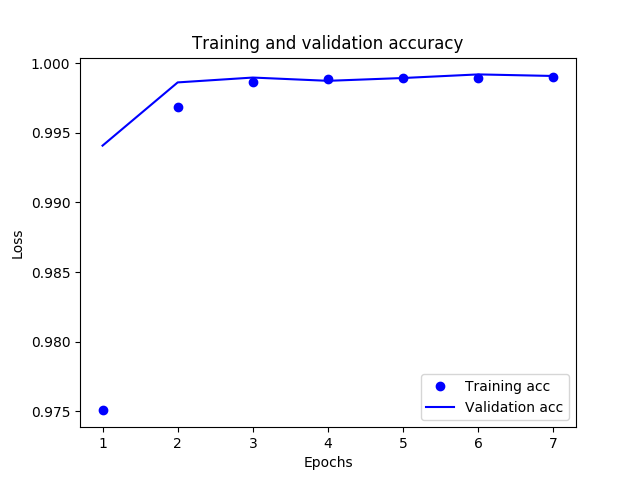
\includegraphics[width=.9\linewidth]{accuracy-train.png}
		\caption{训练与验证accuracy变化}
		\label{fig:acc}
	\end{subfigure}
	\caption{75\%训练-25\%测试的结果}
	\label{fig:test_subfigure}
\end{figure}


这么高的准确率展现了深度学习强大的学习能力。在训练数据集和测试数据集与本实验相同的情况下,陈万志,李东哲等人在文献\cite{r10}中使用了一种将白名单和PSO-BP神经网络过滤有机融合的方法,准确率为87.31\%。文献《基于深度置信网络的入侵检测研究-安琪》中使用了深度置信网络(DBN)达到的准确率为95.55\%\cite{r9}。
  
\subsection{结果分析}

从上面给出的多组对比试验的结果来分析,model1-1的网络参数“24-256-512-256-5”所达到的准确率最高,同时其训练时间也在可接受范围之内。继续增加每层的节点数,准确率下降到了73\%,可见并不是网络节点数越多效果越好。相反,将网络节点数降低一些,却不会发生向增加网络节点数那种情况的准确率大幅度下降,从图表中可知,不同节点数、不同网络层数的情况下,深度学习模型的准确率在90\%-92\%之间浮动。同时可依发现,深度学习模型的参数数量明显影响着深度学习网络的训练速度。

对于batchsize的选择,从实验结果可以发现,在网络结构调整为较为优秀的情况下,batchsize的大小主要影响的是深度学习网络的训练速度。从实验结果的数据中可以发现,batchsize越大,训练速度也就越快。当然batchsize也不能无限的增大,在实验测试时,当我将batchsize设置的非常大时(针对这个数据集,设置了16384),训练速度反而降低了,几乎与batchsize为256时的速度一样,同时,模型的收敛速度也变慢了。这一结果与第三章对mini-batch的分析一致。因此,在应用时,应当根据数据集的规模等因素尝试不同大小的batchsize,直至选择出准确率与训练时间都较好的大小。

对于优化算法的选择,不同模型适合不同的优化算法,在本实验所构建的深度学习模型上,Nadam优化算法的表现最好。同时,RMSprop优化算法也有着不错的表现。在上述实验中,除了优化算法对比试验使用了不同的优化算法,在其它实验中的优化算法都使用了Nadam,下面给出Nadam在本实验中所使用的详细参数供参考。
\begin{itemize}
	\item 学习率lr: 0.002。
	\item beta\_1/beta\_2: 0.9/0.999,通常选取接近于1的数值。
	\item 模糊因子epsilon: None,不使用。
	\item schedule\_decay: 0.004
\end{itemize}

对于二分类与五分类的情况,在不使用Dropout技术时,五分类的准确率较高,达到了92\%以上,然而,二分类的表现很糟糕,只有80\%左右,可见并没有训练好。在加入了Dropout技术并取Dropout值为0.5后,二分类的准确率提高到了92\%以上,和五分类为同一水准。可见,Dropout技术在深度学习的训练上的效果是十分突出的。

在最后,本文也给出了只使用训练数据集进行训练和测试的准确率,这种情况下,测试集不包括未知类型的攻击,都是已知类型的攻击,从结果来看,本文的深度学习模型在这种情况下拟合的非常好,曲线符合一个训练优秀的模型应当展现的曲线。测试的准确率也比文献中的另外两种方法高。

对于训练集和测试集分别使用KDD 10\%训练集和corrected测试集的情况(也是本文大部分实验所使用的情况),在测试集上的准确率最高为92.67\%。可见本文提出的基于深度学习的网络流量异常检测算法模型的检测能力是非常不错的,并且具有不错的泛化能力。

\section{本章小结}

本章是对前面所叙述的基于深度学习的网络流量异常检测算法的实验及实现。首先详细说明了实验数据集各用于训练或是测试环节中,并同时给出了详细的解释。然后给出了实验平台的详细信息,供对比和参考。紧接着分多个部分给出了多组对比试验及其结果,并在最后一部分中对实验结果进行了详细的分析,总结得出的结论。通过本章内容,揭示了本文所提出的算法的应用可能性。